\documentclass[12pt,a4paper,oneside]{book}
\usepackage{comment}
%PL language
\usepackage[QX]{polski}
\usepackage[utf8]{inputenc}
\usepackage[T1]{fontenc}
%\usepackage{polski}
\usepackage{enumitem} % Pakiet do dostosowywania list


\begin{comment}
Aby stworzyć listę numerowaną w LaTeX z wcięciami zgodnymi z językiem polskim, możesz skorzystać z poniższego przykładu:

\documentclass{article}
\usepackage[utf8]{inputenc}
\usepackage[T1]{fontenc}
\usepackage{polski}
\usepackage{enumitem} % Pakiet do dostosowywania list

\begin{document}
	
	\begin{enumerate}[label=\arabic*.,leftmargin=*]
		\item Pierwszy punkt
		\item Drugi punkt
		\item Trzeci punkt
	\end{enumerate}
	
\end{document}

W powyższym kodzie:

label=\arabic*. określa, że elementy listy będą numerowane liczbami arabskimi z kropką na końcu.
leftmargin=* pozwala na dostosowanie lewego marginesu listy, tak aby wcięcia były zgodne z polskimi standardami.
Pakiet enumitem jest bardzo pomocny w dostosowywaniu list, umożliwiając między innymi zmianę stylu numeracji, odstępów między elementami listy oraz wcięć

\end{comment}

\usepackage{latexsym}
\usepackage{tgpagella}
\usepackage{lmodern}
\usepackage{amsmath,amsthm,amsfonts,amssymb,alltt}
\usepackage{epsfig}
\usepackage{pdflscape}
\usepackage{caption}
\usepackage{indentfirst}
\usepackage{float}
%\usepackage{showkeys}
\usepackage{color}
\usepackage{graphicx} % Pakiet do wstawiania obrazów
\usepackage[x11names,dvipsnames,table]{xcolor}
\usepackage{hyperref}
\hypersetup{
pdfauthor={Jakub Trznadel, Mateusz Tęcza, Roman Rusinek nick Theokron},
colorlinks=True,
linkcolor=darkgray,  % color of internal links (change box color with linkbordercolor)
citecolor=BrickRed,  % color of links to bibliography
filecolor=Magenta,   % color of file links
urlcolor=BlueViolet}	%%pdfpagemode=FullScreen}
% diagramy, grafy itp.
\usepackage{tikz}
\usetikzlibrary{positioning}
\usetikzlibrary{arrows}
\usetikzlibrary{arrows.meta}
\usetikzlibrary{chains,fit,shapes,calc}
\tikzset{main node/.style={circle,fill=blue!20,draw,minimum size=1cm,inner sep=0pt}}

\usepackage[linesnumbered,lined,commentsnumbered, algochapter]{algorithm2e}
\SetKwFor{ForEach}{for each}{do}{end for}%
\SetKwFor{ForAll}{for all}{do}{end for}%
\newenvironment{myalgorithm}
{\rule{\textwidth}{0.5mm}\\\SetAlCapSty{}\SetAlgoNoEnd\SetAlgoNoLine\begin{algorithm}}{\end{algorithm}\rule{\textwidth}{0.5mm}}
%---------------------
\overfullrule=2mm
\pagestyle{plain}
\textwidth=15cm \textheight=685pt \topmargin=-25pt \linespread{1.3} 
\setlength{\parskip}{0pt}
\setlength\arraycolsep{2pt}
\oddsidemargin =0.9cm
\evensidemargin =-0.1cm
\captionsetup{width=.95\linewidth, justification=centering}
%---------------------
\usepackage{amssymb}%znak zatwierdzenia "fałka" w tabeli,  $\checkmark$
\usepackage{color}

% --------------------------------------------
% Definicja konwencji wizualnej dla kodu
%\definecolor{mygreen}{rgb}{0,0.6,0}
\definecolor{mygray}{rgb}{0.92,0.92,0.92}
\definecolor{light-gray}{gray}{0.85}
\definecolor{mymauve}{rgb}{0.58,0,0.82}
%\definecolor{myred}{rgb}{1,0,0}


\usepackage{listings}
% wspólny licznik dla figures and lislistings
\makeatletter
\AtBeginDocument{%
  \let\c@figure\c@lstlisting
  \let\thefigure\thelstlisting
  \let\ftype@lstlisting\ftype@figure % give the floats the same precedence
}
\makeatother
%----------------------------------------
\usepackage{listingsutf8}
\renewcommand{\lstlistingname}{Rys.}%{Kod \'{z}r\'{o}d\l{l}owy}
\lstset{
basicstyle=\ttfamily ,
language=python,
inputencoding=utf8/cp1250,
extendedchars=true,
numbers=left, %eller none
numberstyle=\scriptsize\color{black}\bfseries,
%frame = tb,
captionpos = rb,
backgroundcolor=\color{light-gray},
xleftmargin=\parindent,
% xrightmargin=3.5cm
showstringspaces=false,
commentstyle=\color{Red},
keywordstyle=\color{YellowOrange},
keywordstyle=[2]\color{RedViolet},
keywords={and,del,from,not,while,as,elif,global,or,with,assert,else,if,pass,yield,break,
except,import,class,exec,in,raise,continue,finally,is,return,def,for,lambda,try},
keywords=[2]{print,object,type,input,sum,min,max,int,float,str,list,dict,set,tuple},
rulesepcolor=\color{Blue},
escapeinside={<@}{@>},
stringstyle=\color{OliveGreen},
%basicstyle=\color{Black},
%morecomment=[l]\#,%
morestring=[d]{\\'},
morestring=[d]{\\"},
%morestring=[b]',%
%morestring=[b]",%
%morestring=*[d]',%
%morestring=*[d]",%
%morestring=[d]{\\'},
%morestring=**[d]{"},
%morestring=[d]{\\"},
morestring=[s]{'}{'},
morestring=[s]{"}{"},
morestring=[s]{'''}{'''},
morestring=[s]{"""}{"""},
morestring=[s]{f"""}{"""},
morestring=[s]{r"""}{"""},
morestring=[s]{f"}{"},
morestring=[s]{f'}{'},
morestring=[s]{r"}{"},
morestring=[s]{r'}{'},
morecomment=[s]{Traceback}{Error*},
literate={ą}{{\k{a}}}1
             {Ą}{{\k{A}}}1
             {ę}{{\k{e}}}1
             {Ę}{{\k{E}}}1
             {ó}{{\'o}}1
             {Ó}{{\'O}}1
             {ś}{{\'s}}1
             {Ś}{{\'S}}1
             {ł}{{\l{}}}1
             {Ł}{{\L{}}}1
             {ż}{{\.z}}1
             {Ż}{{\.Z}}1
             {ź}{{\'z}}1
             {Ź}{{\'Z}}1
             {ć}{{\'c}}1
             {Ć}{{\'C}}1
             {ń}{{\'n}}1
             {Ń}{{\'N}}1
}



% --------------------------------------------

\usepackage{verbatim} %do objęcia komentarzem wiele liniii w latex, współdział 
\newtheorem{tw}{Twierdzenie}[chapter]
\newtheorem{lem}[tw]{Lemat}
\newtheorem{co}[tw]{Wniosek}
\newtheorem{prop}[tw]{Stwierdzenie}
\theoremstyle{definition}
\newtheorem{ex}{Przykład}
\newtheorem{re}[tw]{Uwaga}
\newtheorem{de}{Definicja}[chapter]
\newcommand{\bC}{{\mathbb C}}
\newcommand{\bR}{{\mathbb R}}
\newcommand{\bZ}{{\mathbb Z}}
\newcommand{\bQ}{{\mathbb Q}}
\newcommand{\bN}{{\mathbb N}}
\newcommand{\captionT}[1]{\caption{\textsc{\footnotesize{#1}}}}
\renewcommand\figurename{Rys.}
\newcommand{\Csharp}{C\raisebox{0.5ex}{\tiny\textbf{\#}}} %znak C# po 
\numberwithin{equation}{chapter}
\renewcommand{\thefootnote}{\arabic{footnote})}
%\renewcommand{\thefootnote}{\alph{footnote})}

 %\usepackage[maxcitenames=3]{biblatex}
 
\usepackage[polish]{babel}
%\usepackage{biblatex}

\begin{document}

% --------------------------------------------
% Strona tytułowa
% --------------------------------------------

\begin{titlepage}
%\thispagestyle{empty}
\begin{center}
{\Large \textbf{Collegium Witelona Uczelnia Państwowa}}\\[0.2cm]

\includegraphics[scale=0.35]{images/witelon.png}\\[1cm]
{\large \textbf{Wydział Nauk Technicznych i Ekonomicznych}}\\[0.2cm]
Kierunek: INFORMATYKA\\[0.2cm]
specjalność: Projektowanie aplikacji mobilnych i internetowych\\[1cm]
 
% Title

{\LARGE \textbf{Sprawozdanie\\Platforma Internetowa   "AMORA"~~w. 1.0.0} \\[8.0cm] }

 %\begin{comment}
% Author and supervisor
\noindent
\begin{minipage}[t]{0.5\textwidth}
	\textbf{Skład zespołu projektowego:}\\
	Roman Rusinek~~- nr albumu: 43257\\
	Mateusz Tęcza  ~~- nr albumu: 43263\\
	Jakub Trznadel ~- nr albumu: 42765\\
	

\end{minipage}%
\begin{minipage}[t]{0.5\textwidth}
	\begin{flushright}
		\begin{tabbing}
			\hspace*{2cm}\= \kill
			\textbf{Projekt programistyczny}\\
			\text{prowadzony pod kierunkiem}\\
			\text{mgr inż. Krzysztof Rewak}
		\end{tabbing}
	\end{flushright}
\end{minipage}
%\end{comment}

\vfill

% Bottom of the page
{\large Legnica \the\year}

\end{center}
\end{titlepage}

\addtocontents{toc}{\protect\thispagestyle{empty}} %wyłaczenie numeracji stron spisu tresci
\pagestyle{empty}

%\thispagestyle{empty}
\section*{Streszczenie}
 Projekt randkowej platformy internetowej, kojarzącej ze sobą osoby przeciwnej płci.
 Wersja 1.0.0 Projektu "Amora"~~obsługuje języki: angielski i polski.

\section*{Abstract}
A project for an online dating platform that matches people of the opposite sex with each other.
Version 1.0.0 of Project "Amora"~~supports English and Polish languages.
% --------------------------------------------
% Spis treści
\tableofcontents
% --------------------------------------------
\newpage
% --------------------------------------------
% Wstęp. Postawienie zagadnień                          
% --------------------------------------------
%\chapter*{Wstęp} 
%\addcontentsline{toc}{chapter}{Wstęp}
% --------------------------------------------
% Rozdział 1. Preliminaria 
% --------------------------------------------

\chapter{Wstęp}
Zadaniem projektu programistycznego  "Amora" jest zbudowanie platformy internetowej, kojarzącej  osoby przeciwnej płci  w pary. Projekt jest realizowany zgodnie z filozofią MVP - Minimum Viable Product, czyli staramy się zaprojektować system o minimalnej użyteczności ale o cechach, które pozwolą już go testować, oceniać przez zainteresowanego tym produktem użytkownika. Po zebraniu opinii od użytkowników, można projekt rozbudowywać  rozszerzając istniejące funkcjonalności albo poprzez dołączania całkiem innych.

\setcounter{page}{1}
\section{Podział prac w zespole}
\noindent
Podział prac w zespole:
\begin{itemize}
	\item[--] Jakub Trznadel - frontend (HTML, framework CSS)
	\item[--] Mateusz Tęcza - MVC
	\item[--] Roman Rusinek - opracowanie dokumentacji i bazy danych
\end{itemize}
\newpage
\chapter{Opis funkcjonalny systemu}
\noindent
Cel:  opracowanie i wdrożenie aplikacji randkowej "AMORA" ułatwiającej kojarzenie w pary.\\
\begin{figure}
	\centering
	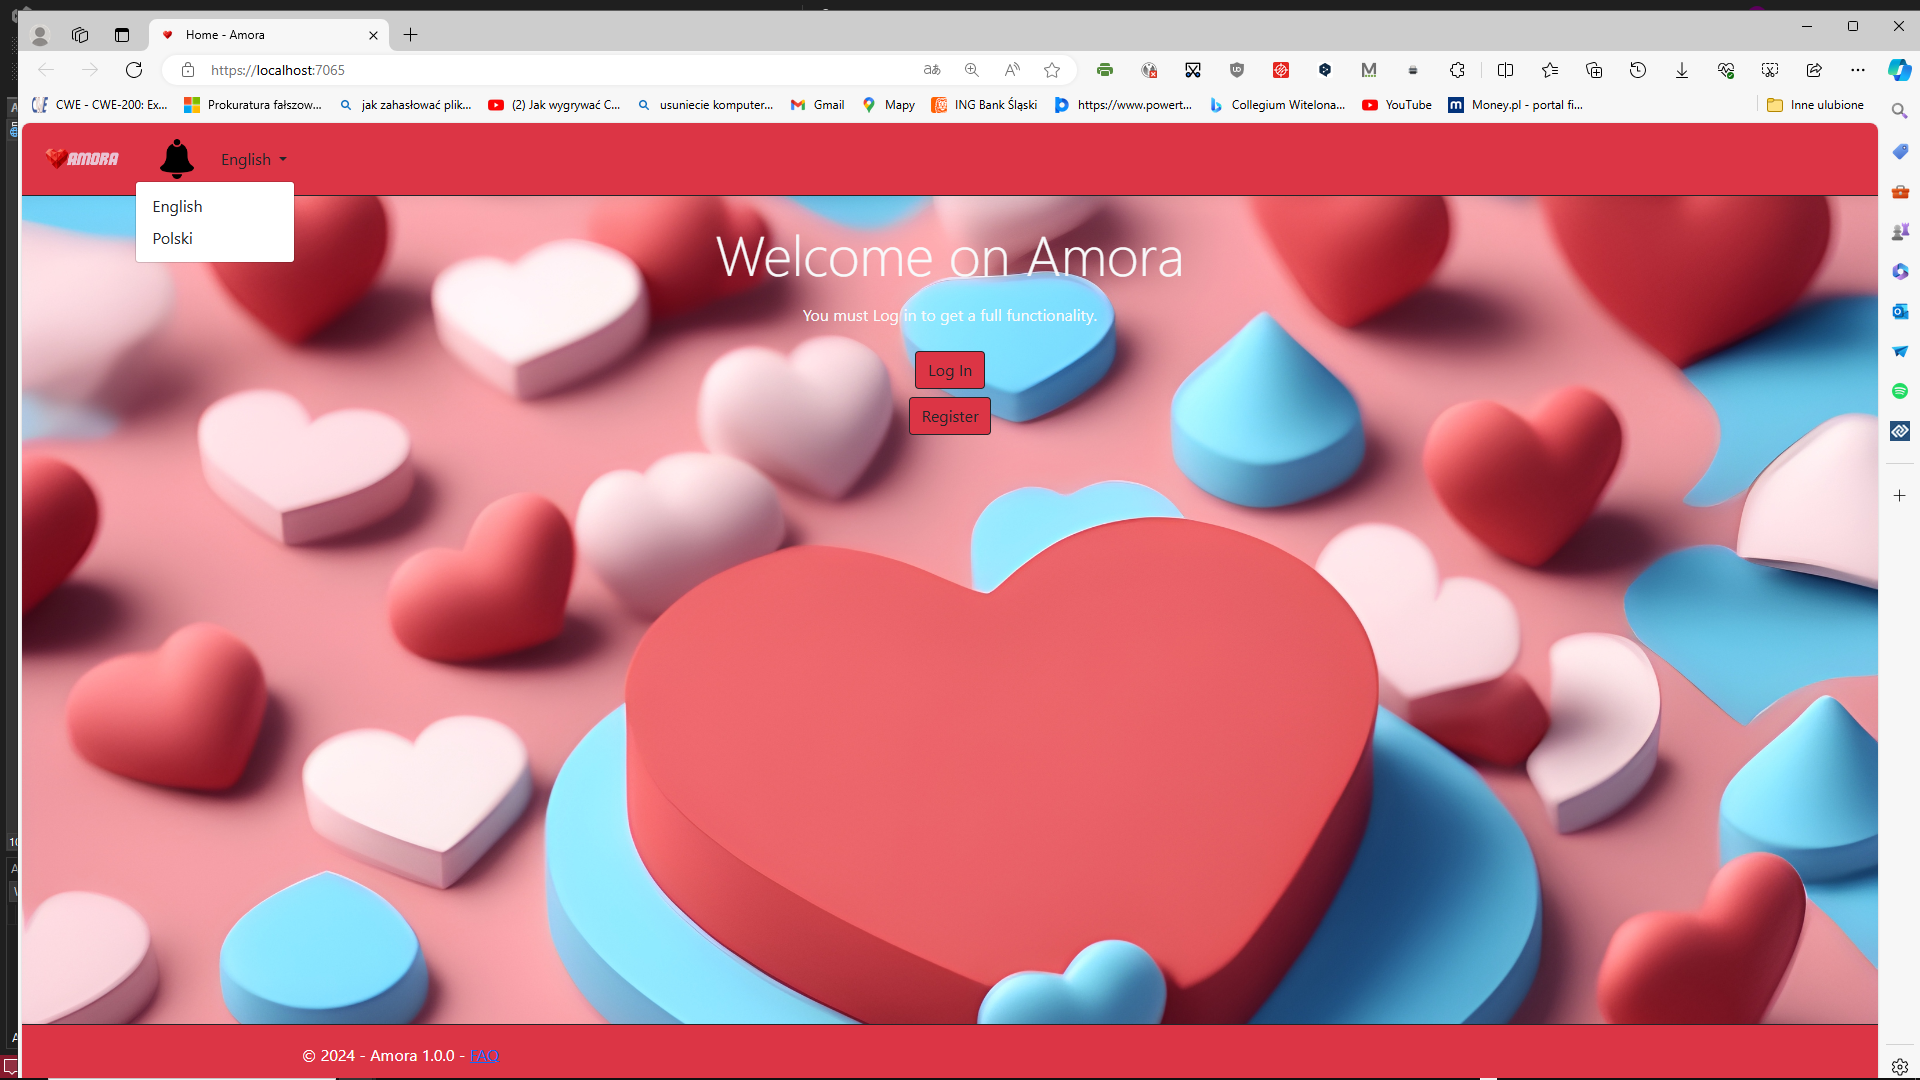
\includegraphics[width=1.0\linewidth]{images/01}
	\caption{}
	\label{fig:01}{Strona początkowa - wybor języka}
\end{figure}
Cel:  opracowanie i wdrożenie aplikacji randkowej "AMORA" ułatwiającej kojarzenie w pary.\\
\begin{figure}
	\centering
	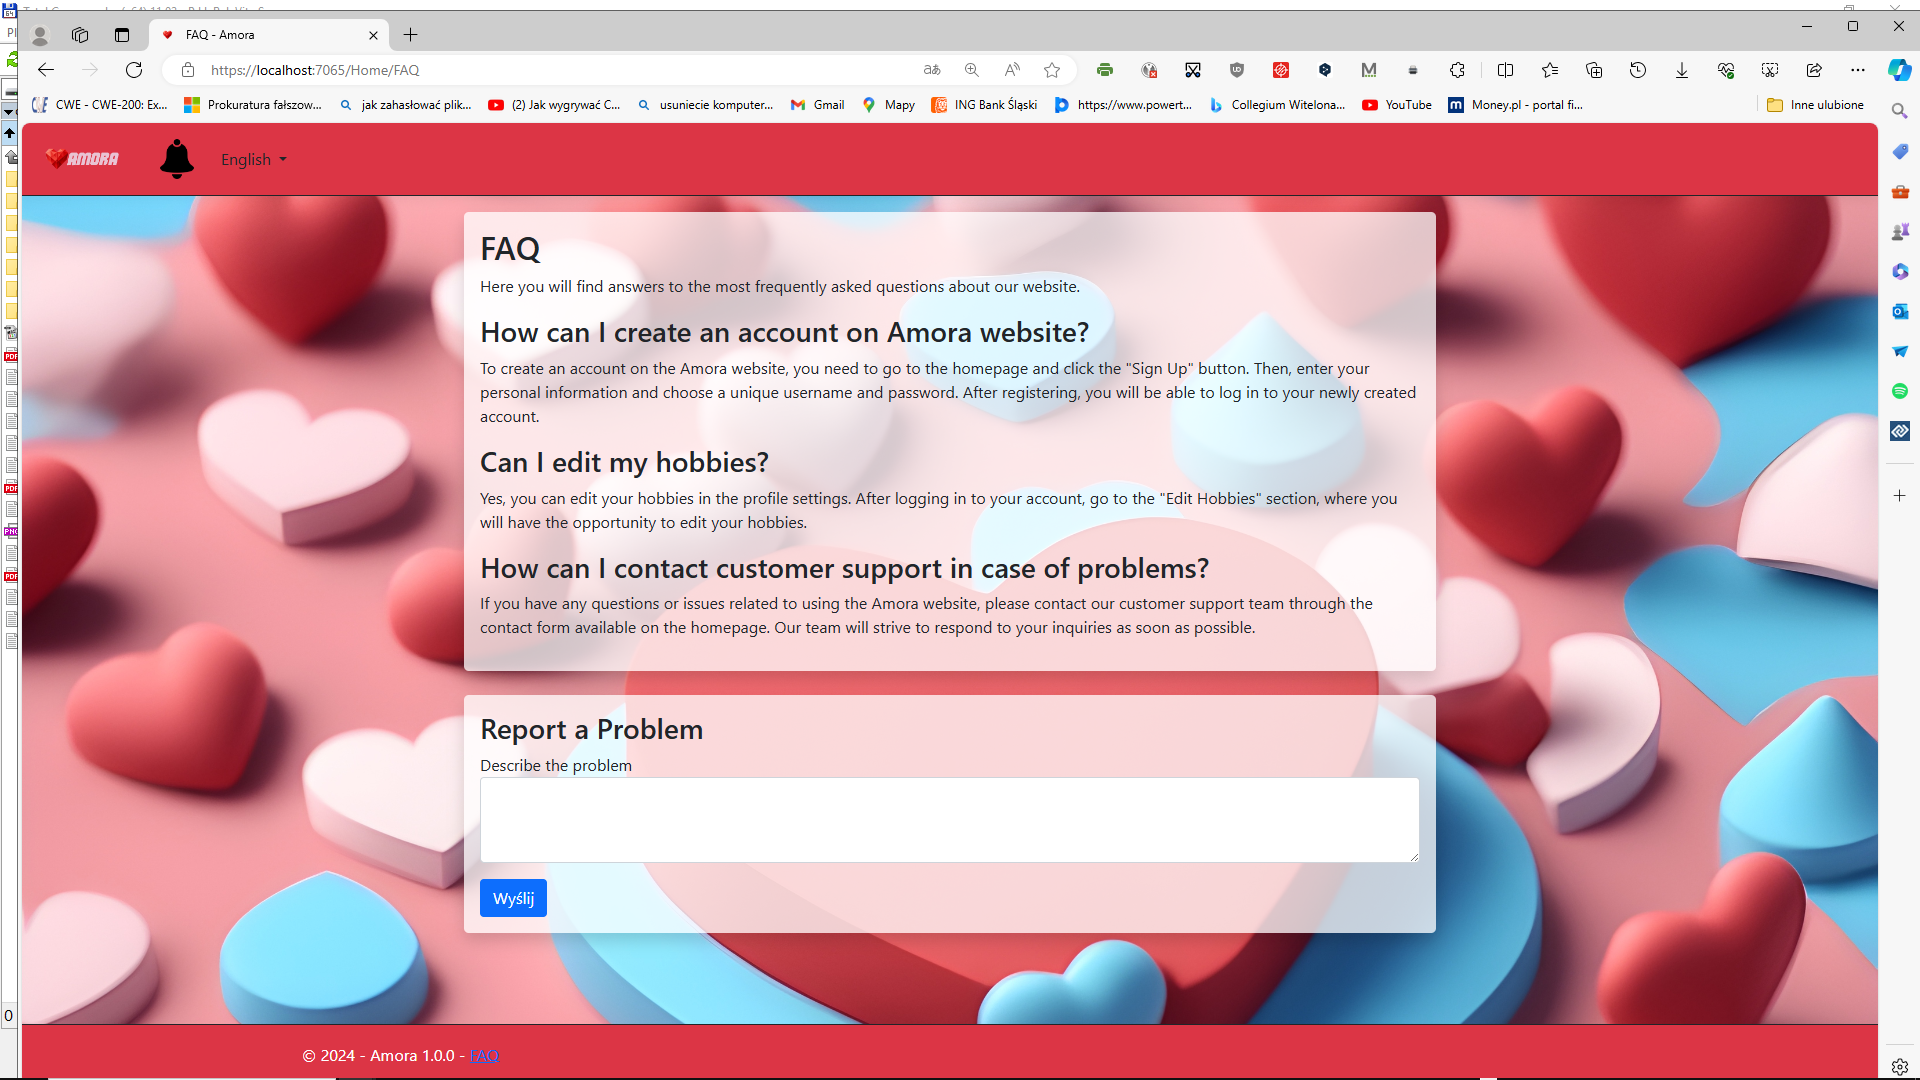
\includegraphics[width=1.0\linewidth]{images/02}
	\caption{}
	\label{fig:02}{Strona początkowa - Przegląd FAQ}
\end{figure}
\begin{figure}
	\centering
	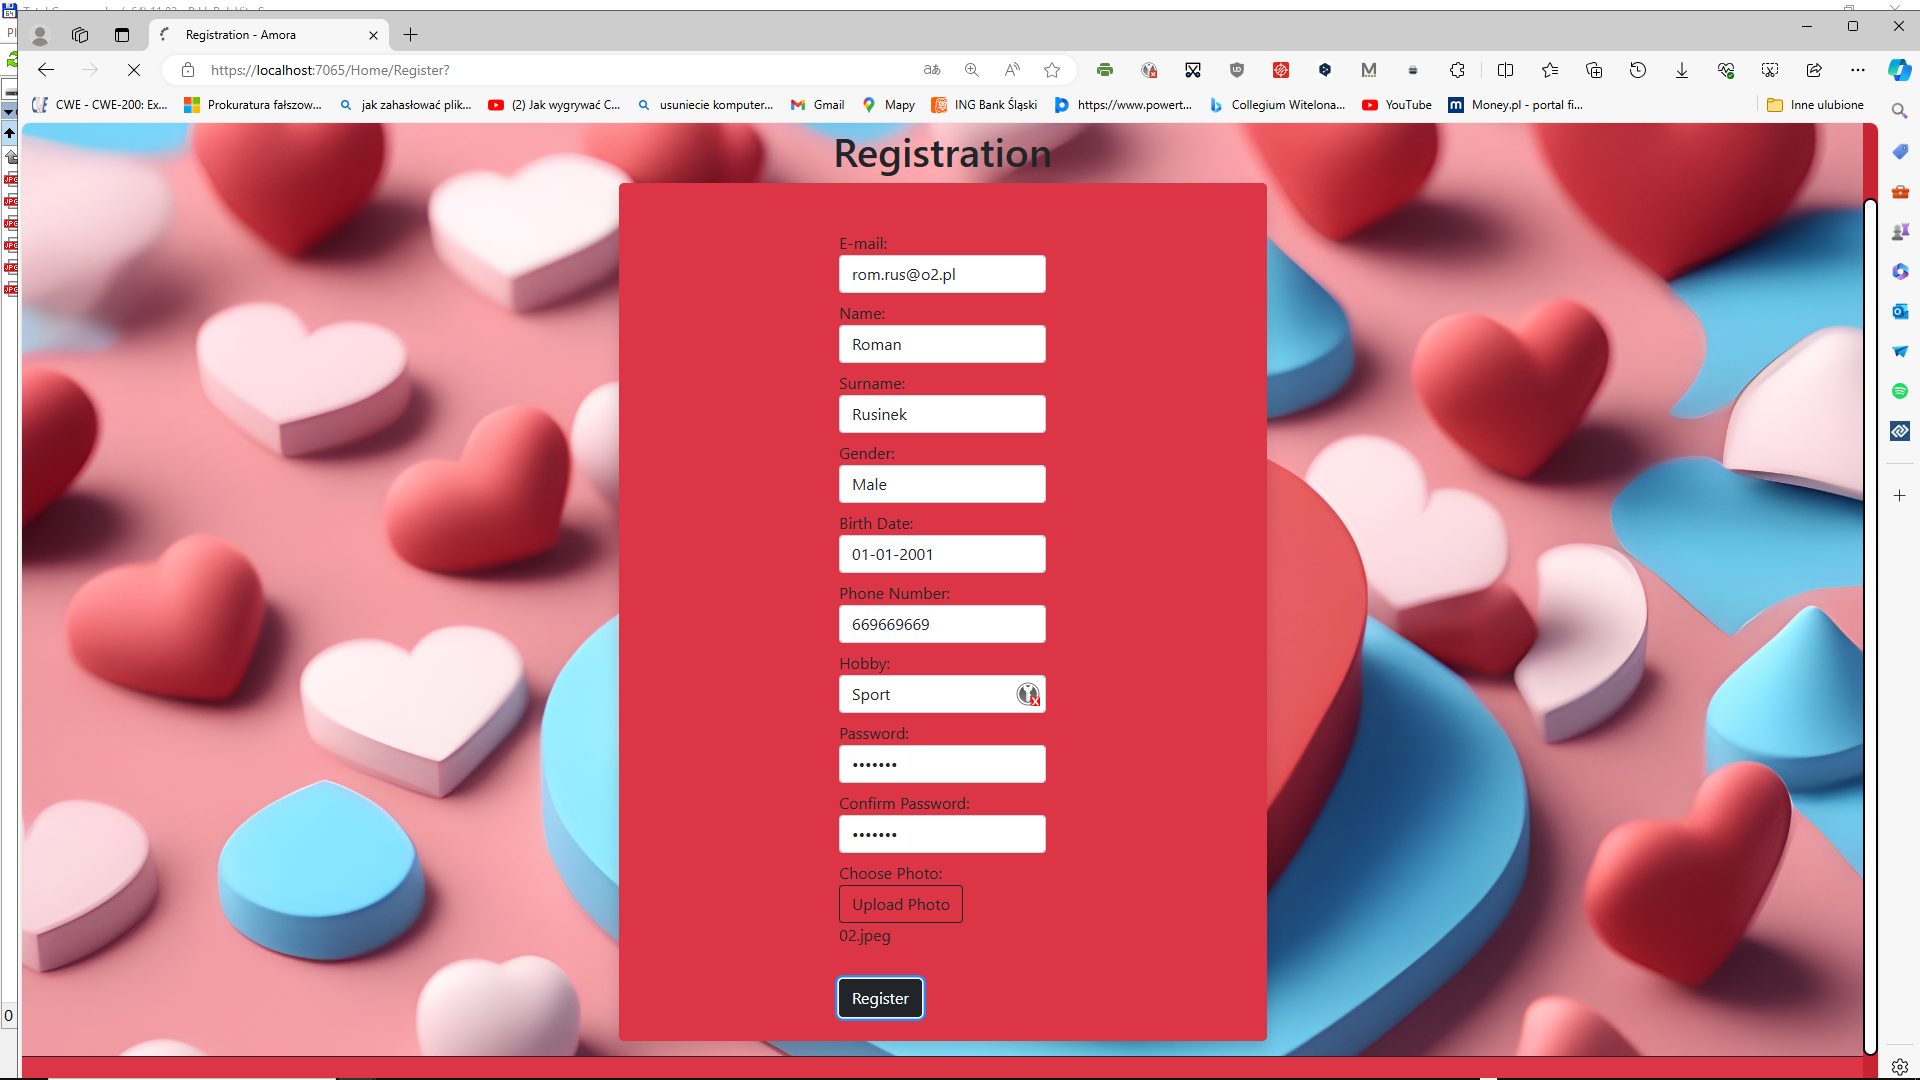
\includegraphics[width=1.0\linewidth]{images/03}
	\caption{}
	\label{fig:03}{Rejestracja}
\end{figure}
\begin{figure}
	\centering
	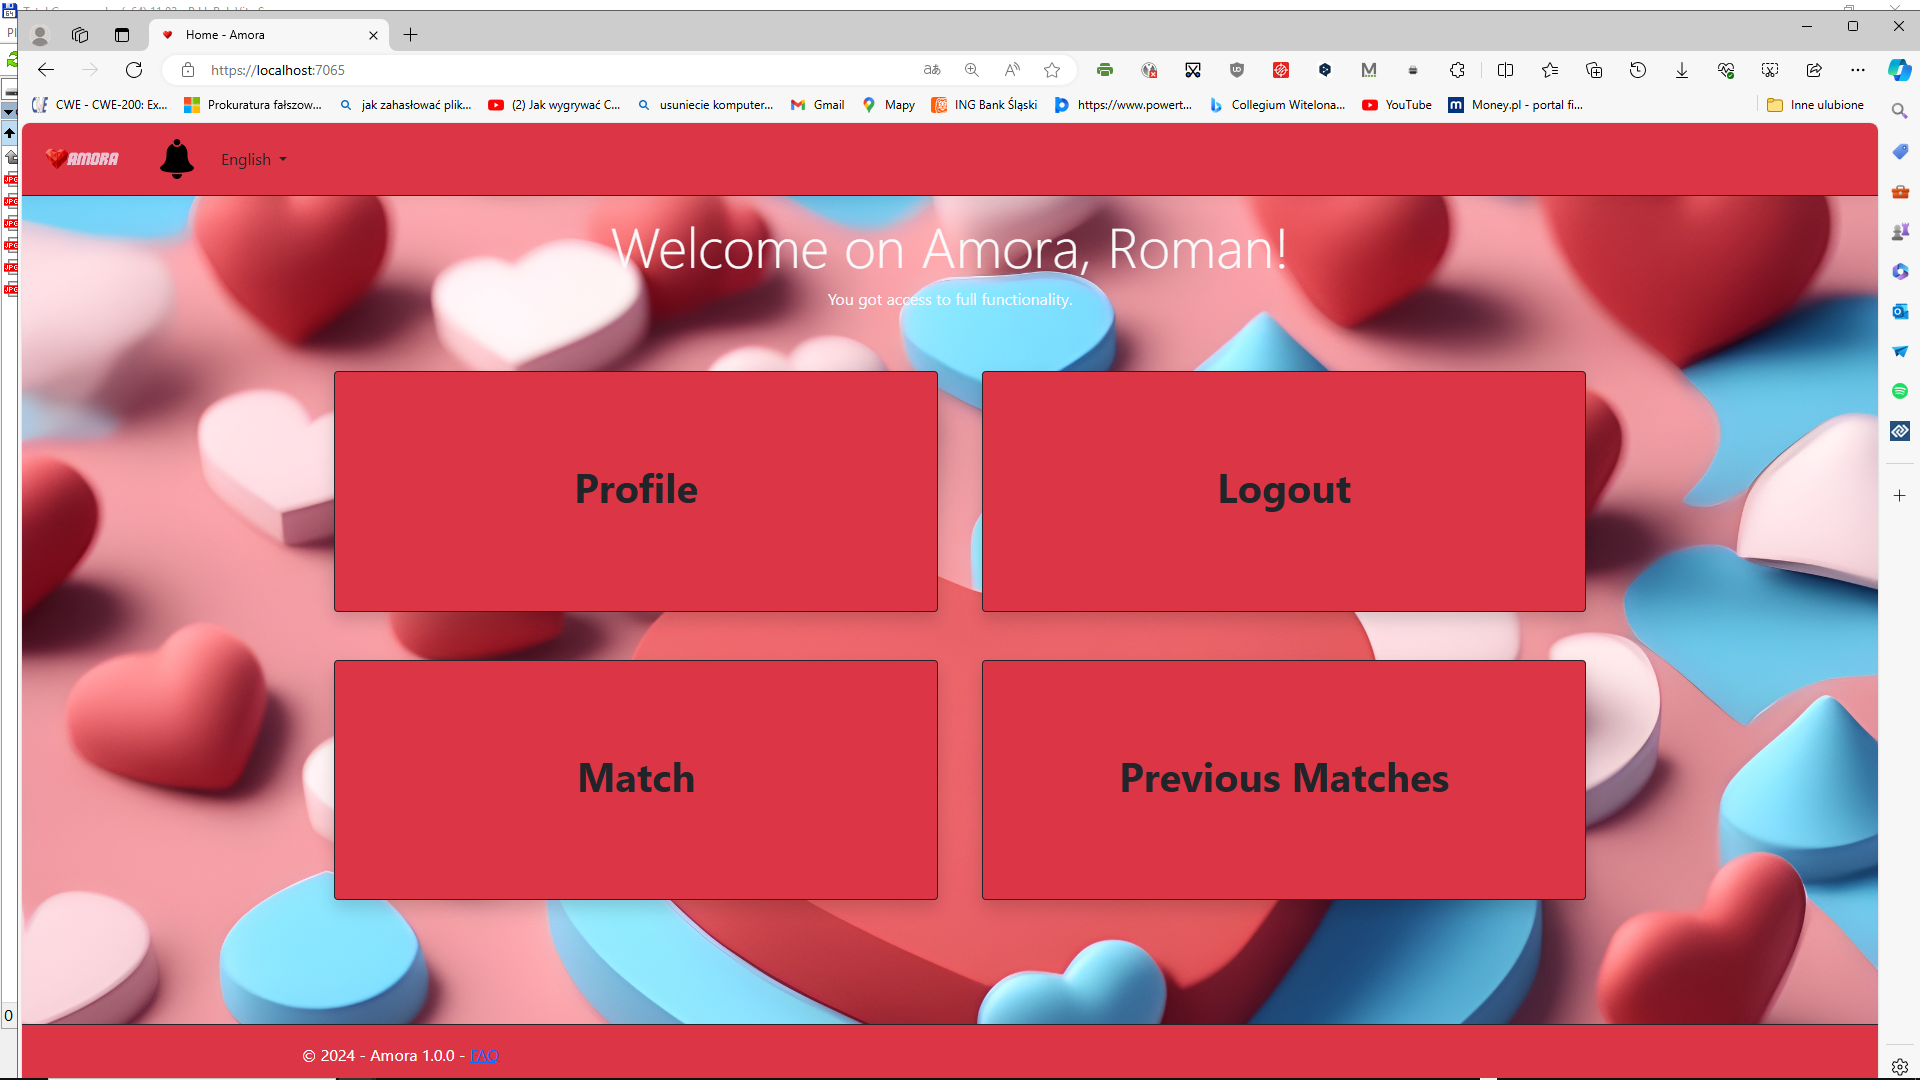
\includegraphics[width=1.0\linewidth]{images/04}
	\caption{}
	\label{fig:04}{Opcje użytkownika}
\end{figure}
\begin{figure}
	\centering
	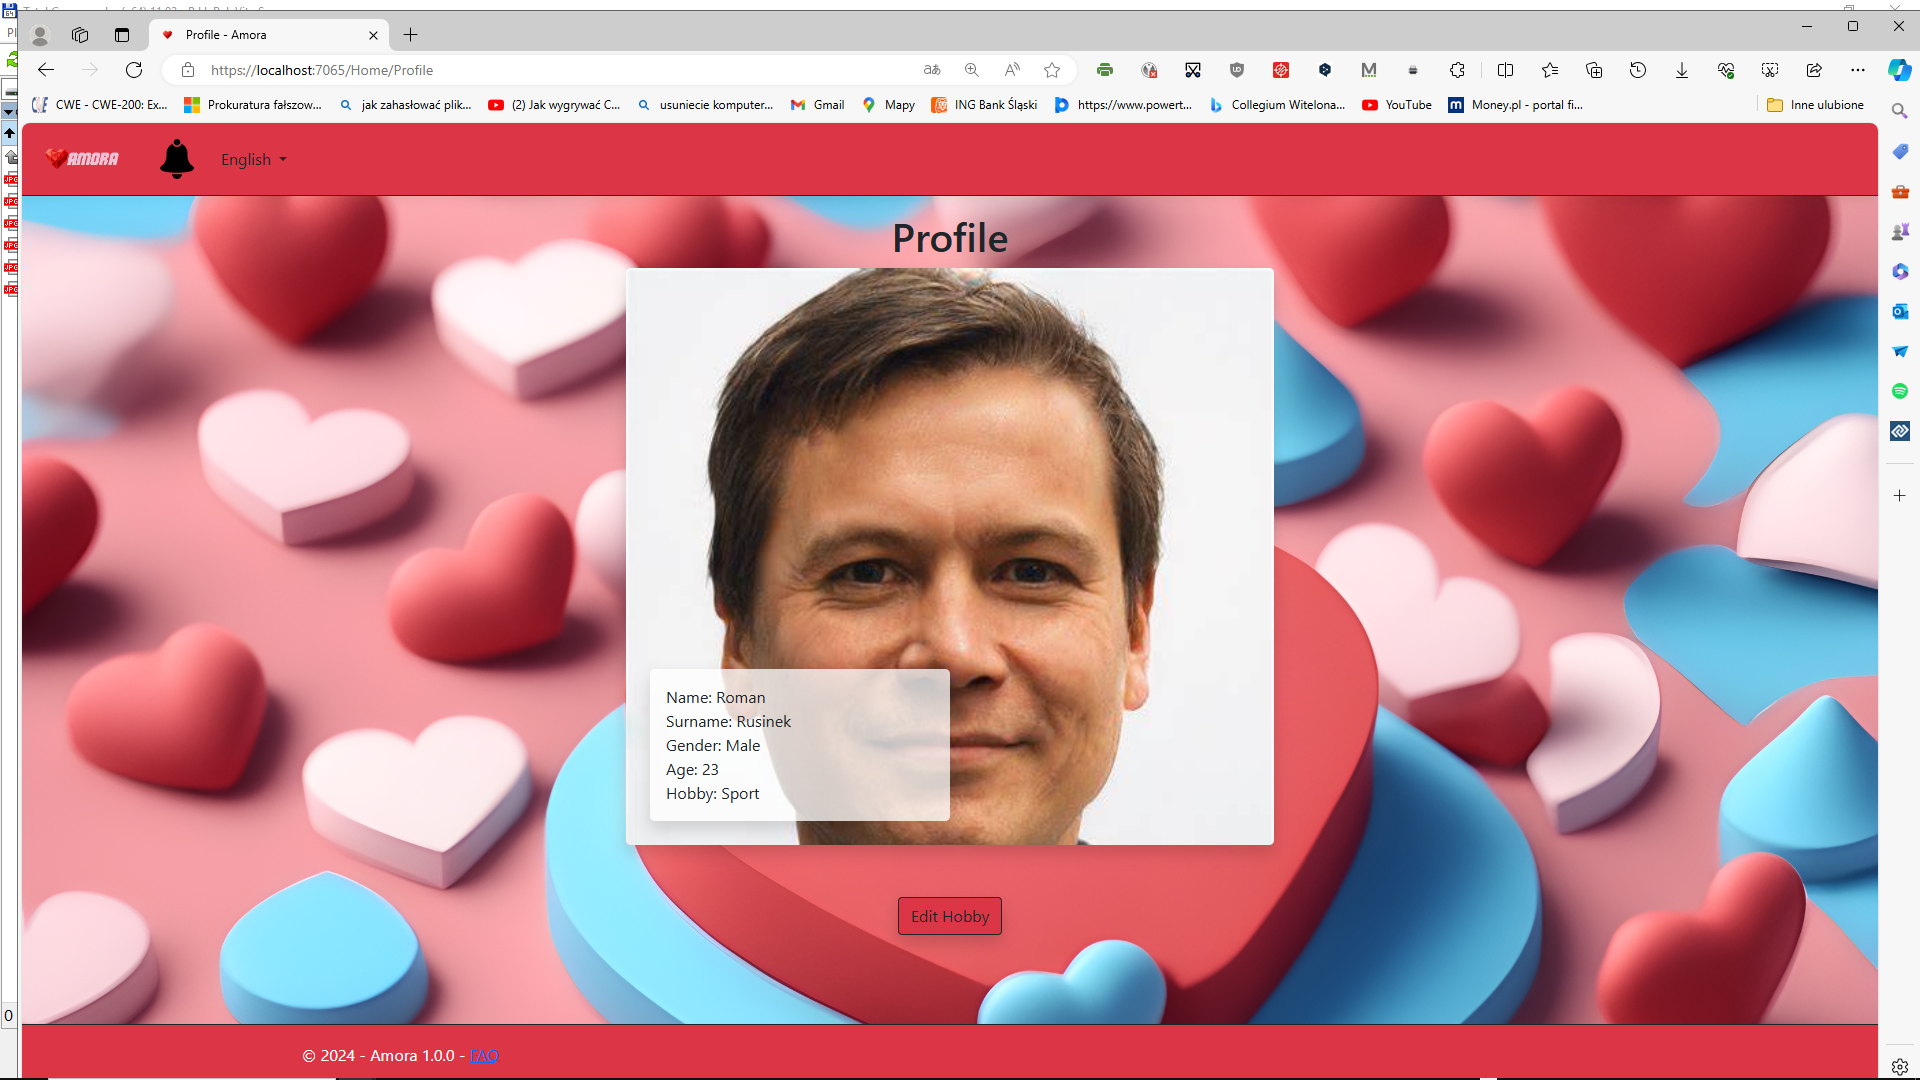
\includegraphics[width=1.0\linewidth]{images/05}
	\caption{}
	\label{fig:05}{Zdjęcie profilowe użytkownika Roman}
\end{figure}
\begin{figure}
	\centering
	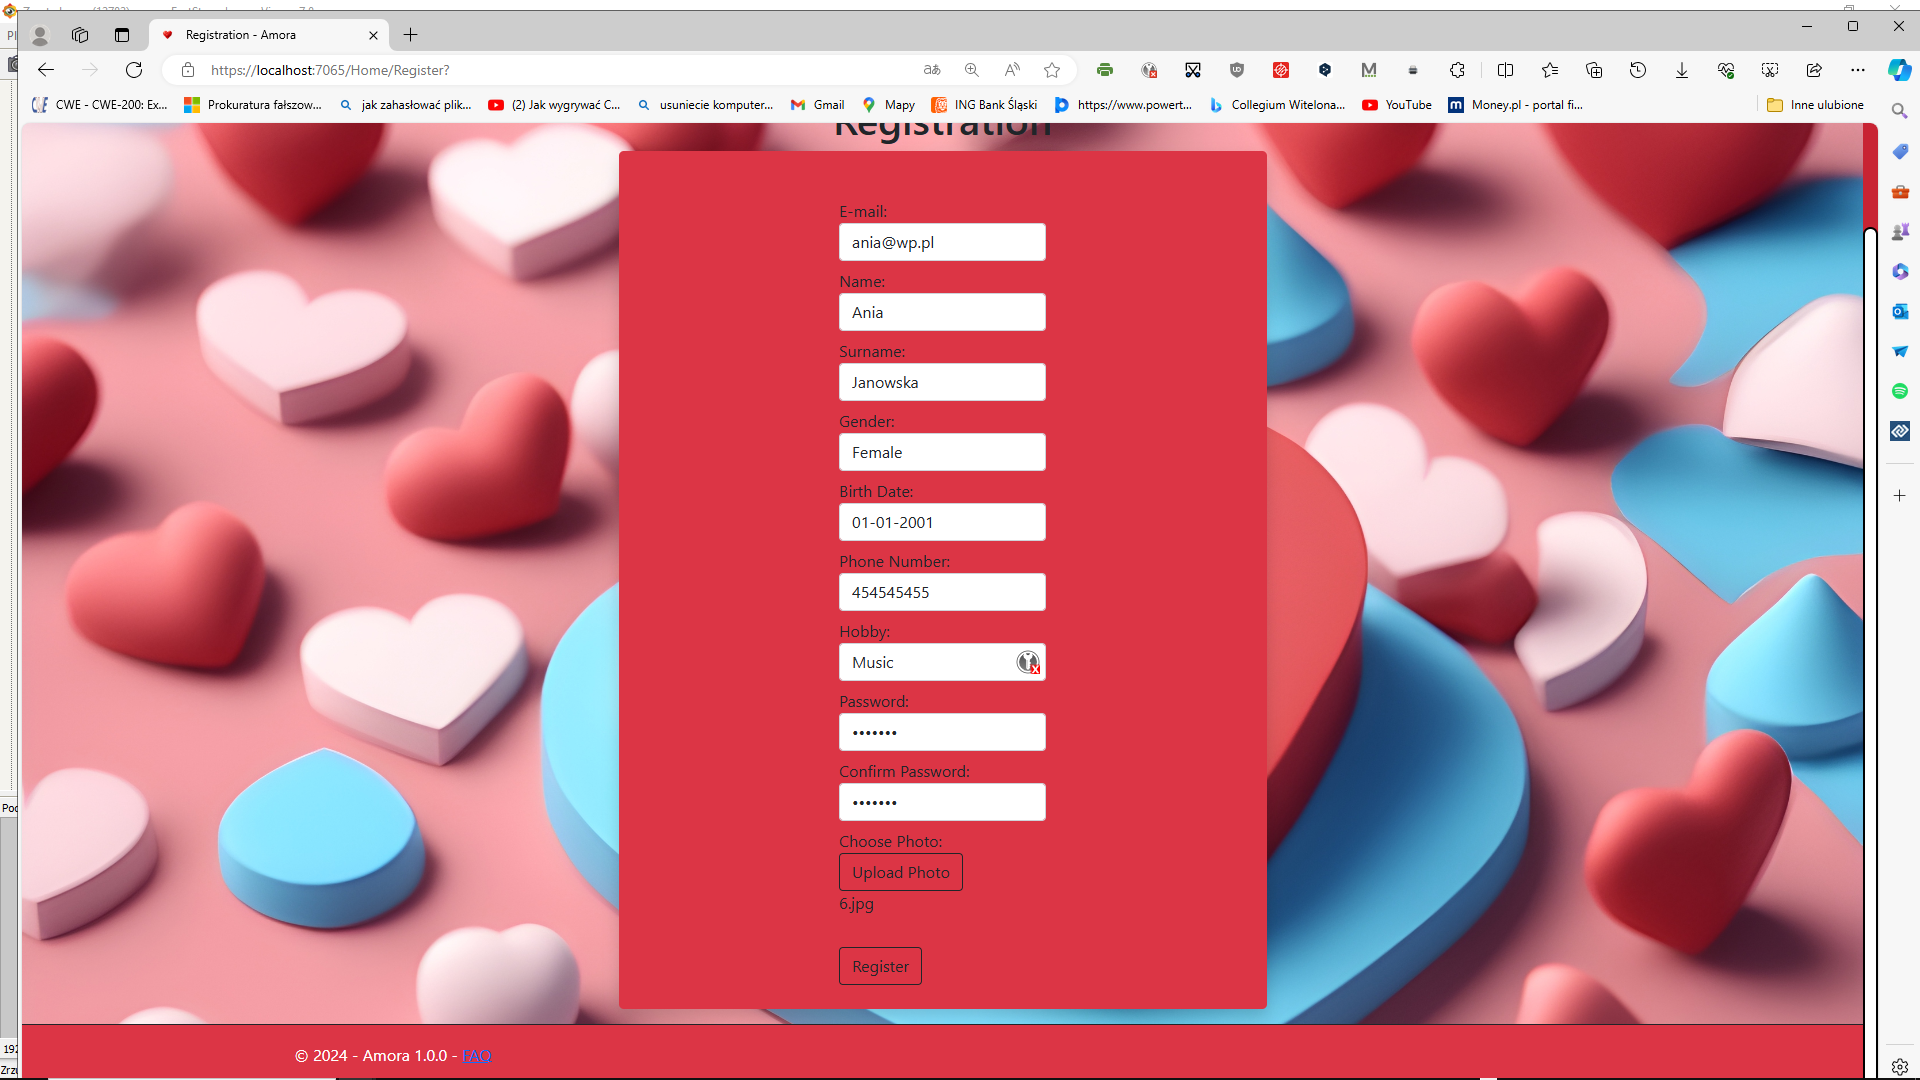
\includegraphics[width=1.0\linewidth]{images/06}
	\caption{}
	\label{fig:06}{Rejjestracja użytkownika Ania}
\end{figure}
\begin{figure}
	\centering
	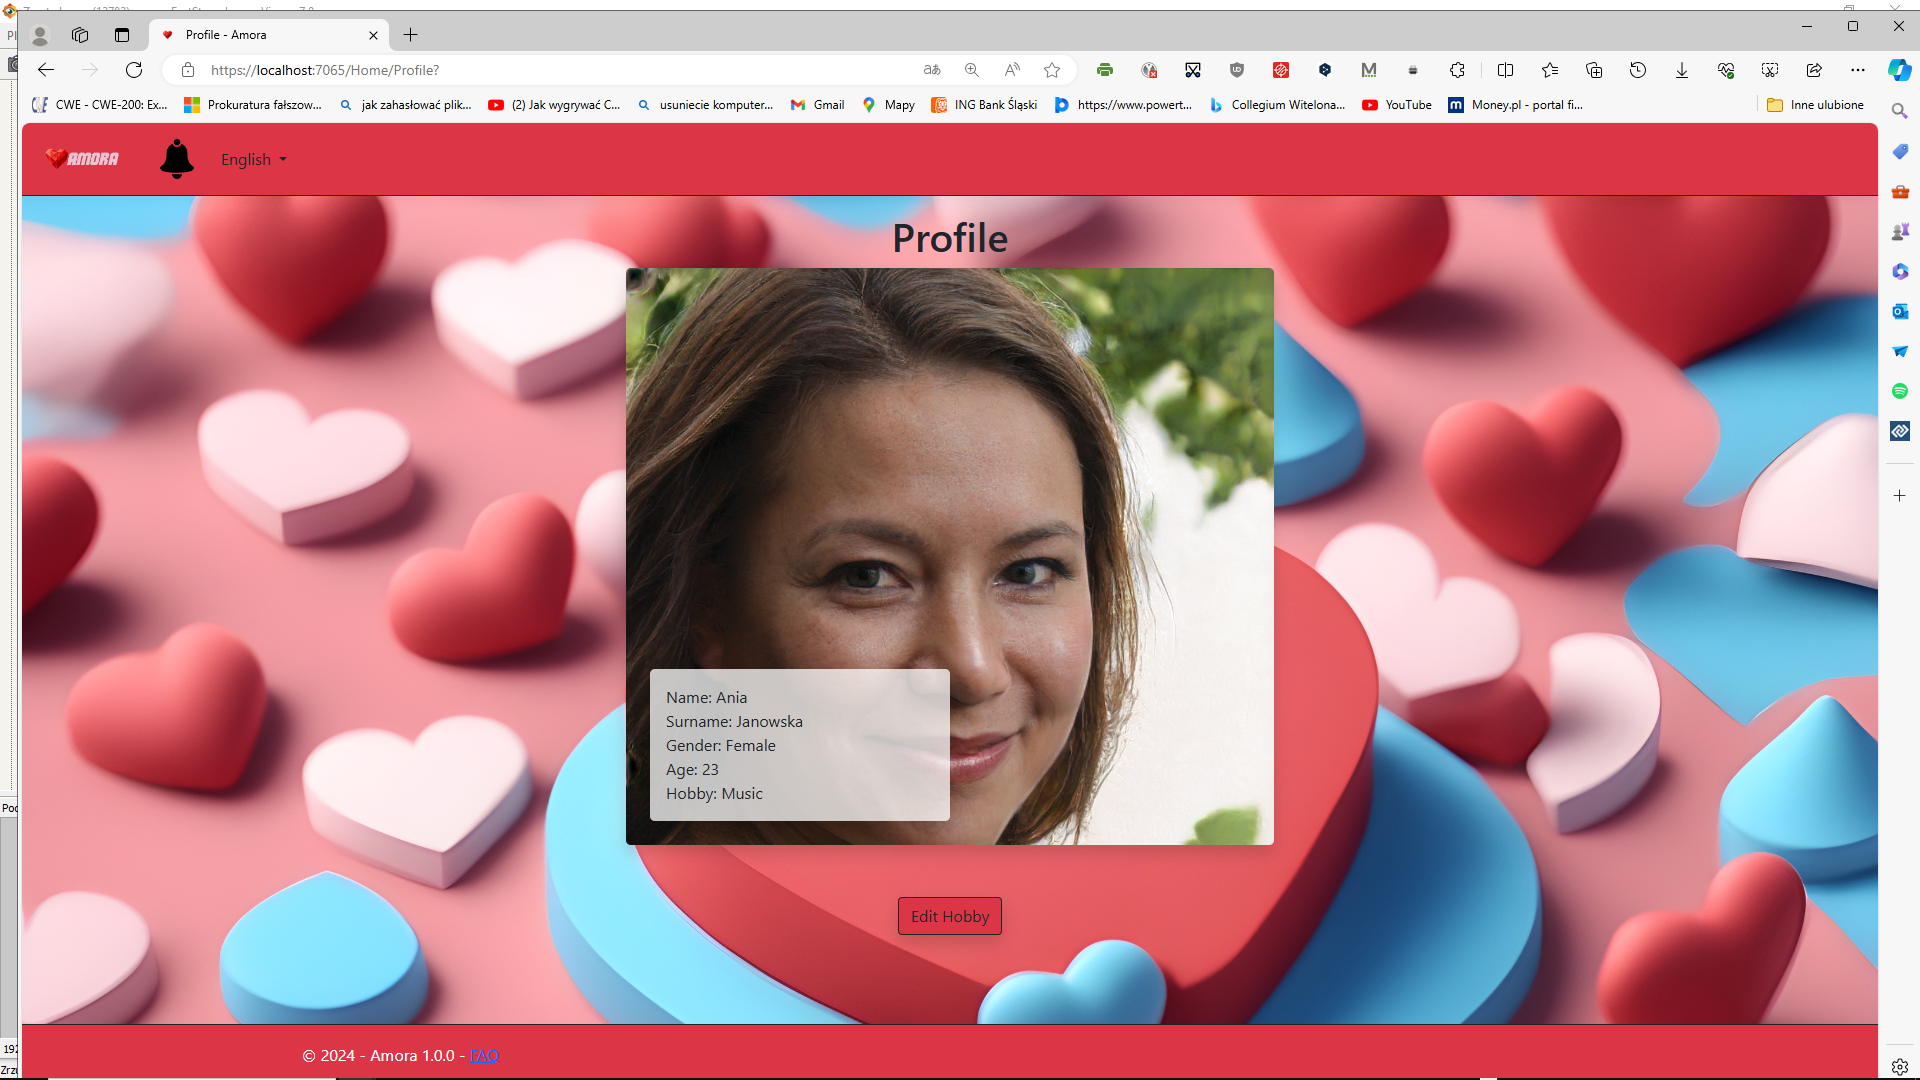
\includegraphics[width=1.0\linewidth]{images/07}
	\caption{}
	\label{fig:07}{Profil użytkownika  Ania}
\end{figure}
\begin{figure}
	\centering
	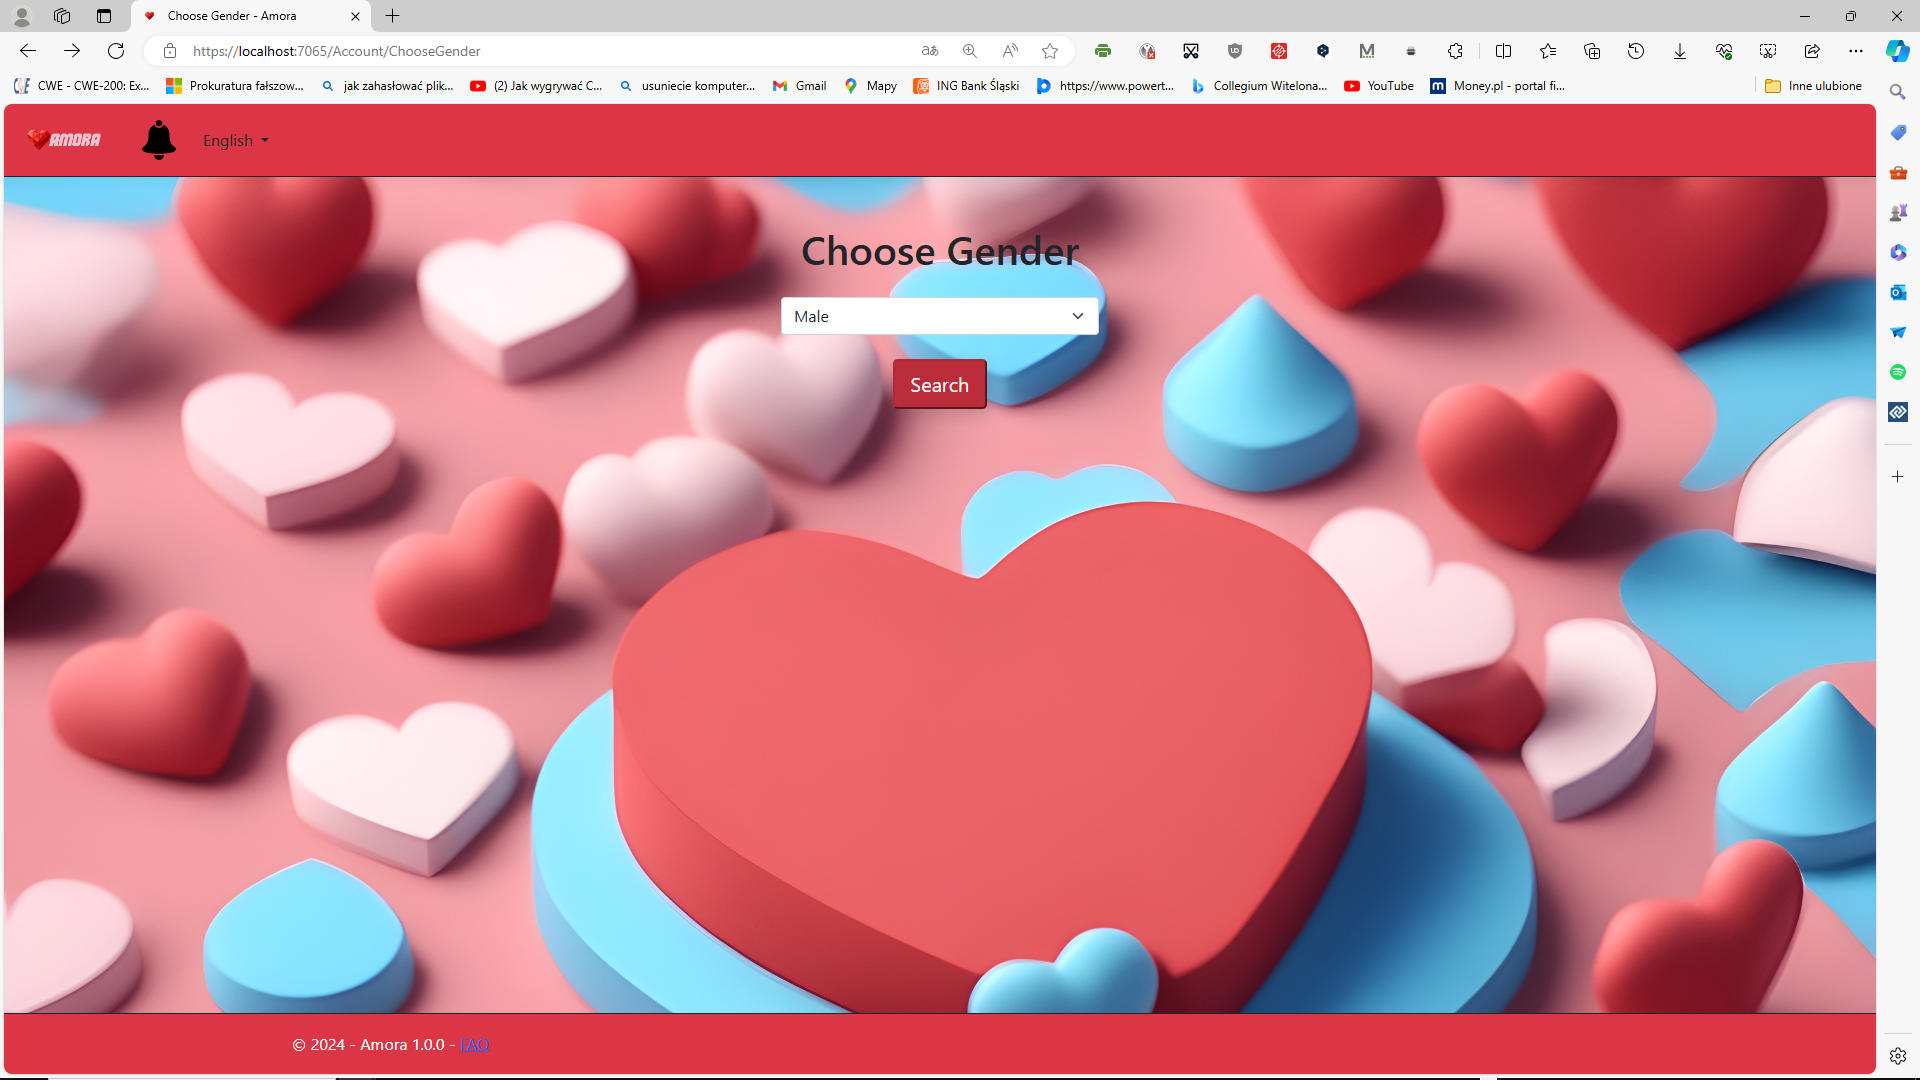
\includegraphics[width=1.0\linewidth]{images/08}
	\caption{}
	\label{fig:08}{Wyszukiwanie przez Anię partnerów}
\end{figure}
\begin{figure}
	\centering
	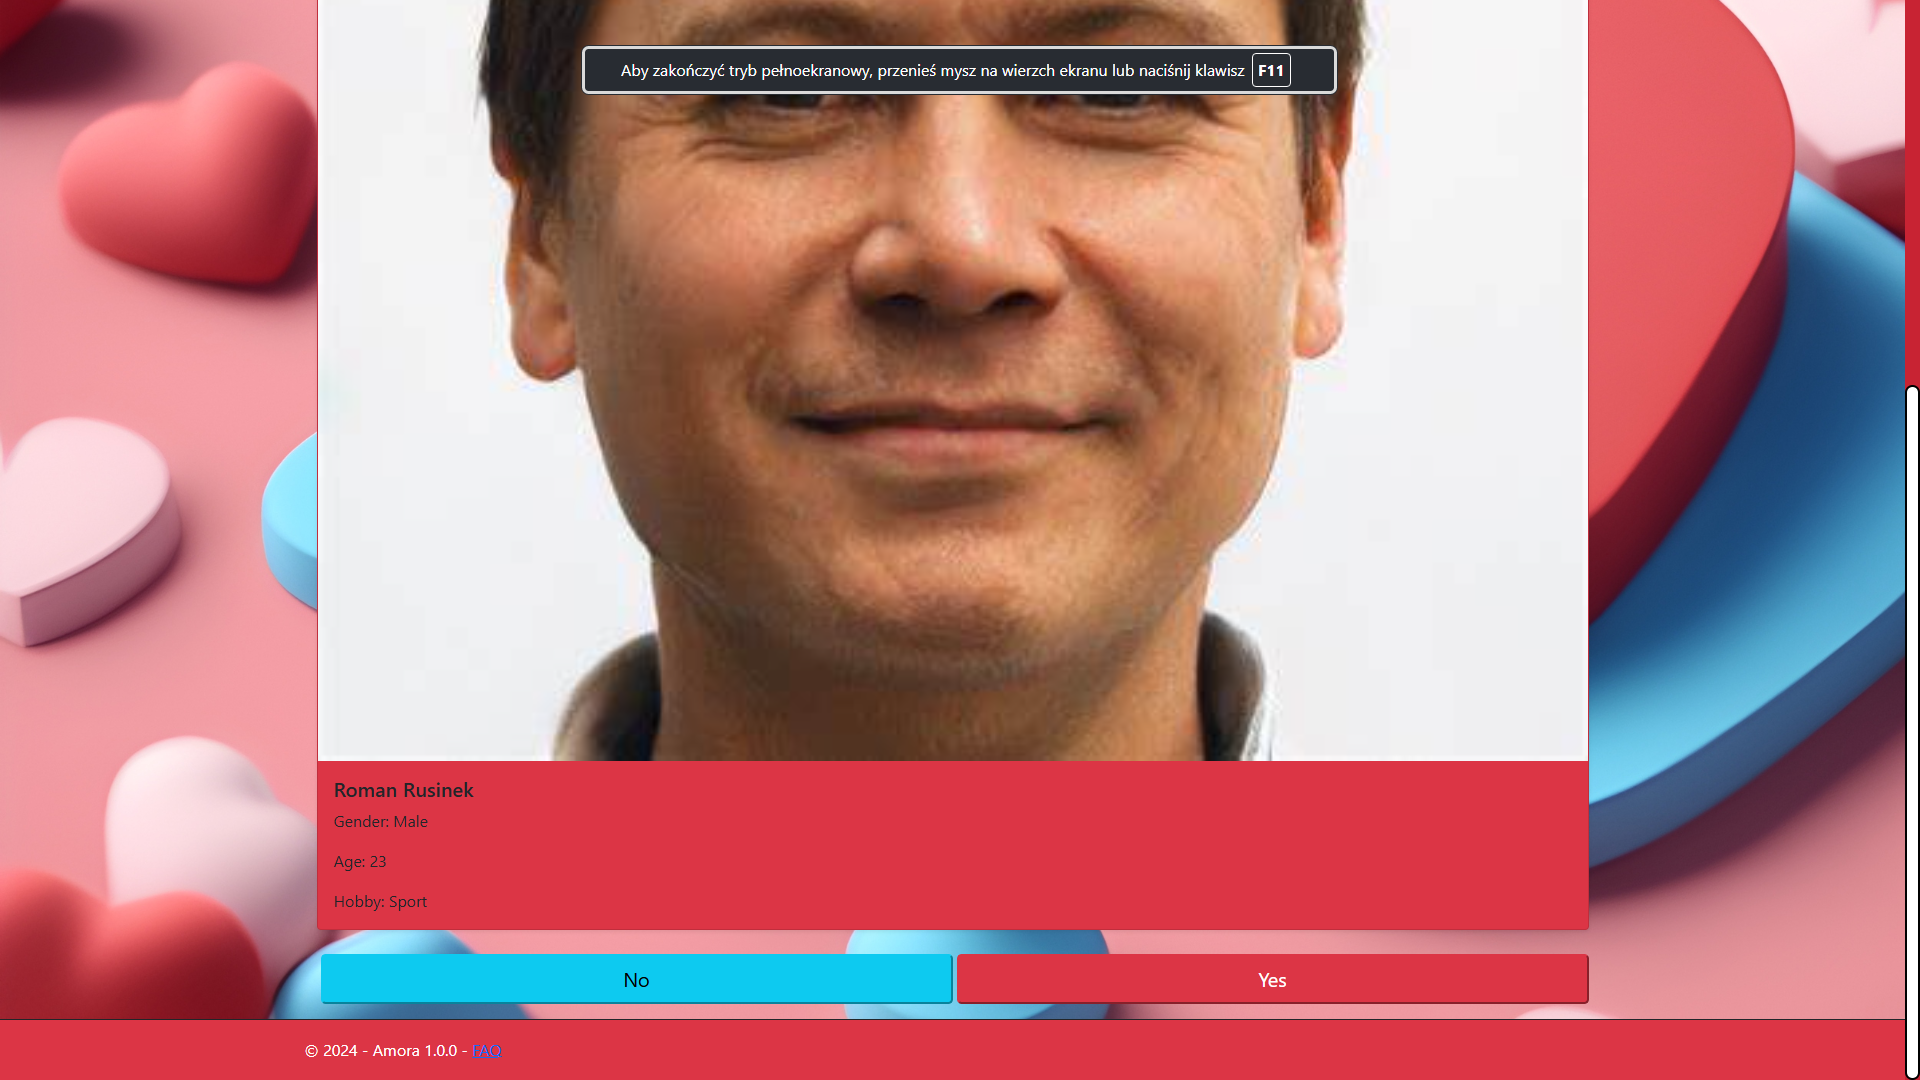
\includegraphics[width=1.0\linewidth]{images/09}
	\caption{}
	\label{fig:09}{Wynik wyszukiwania Ani-znaleziono jedną propozycje znajomości z użytkownikiem Romanem}
\end{figure}
\begin{figure}
	\centering
	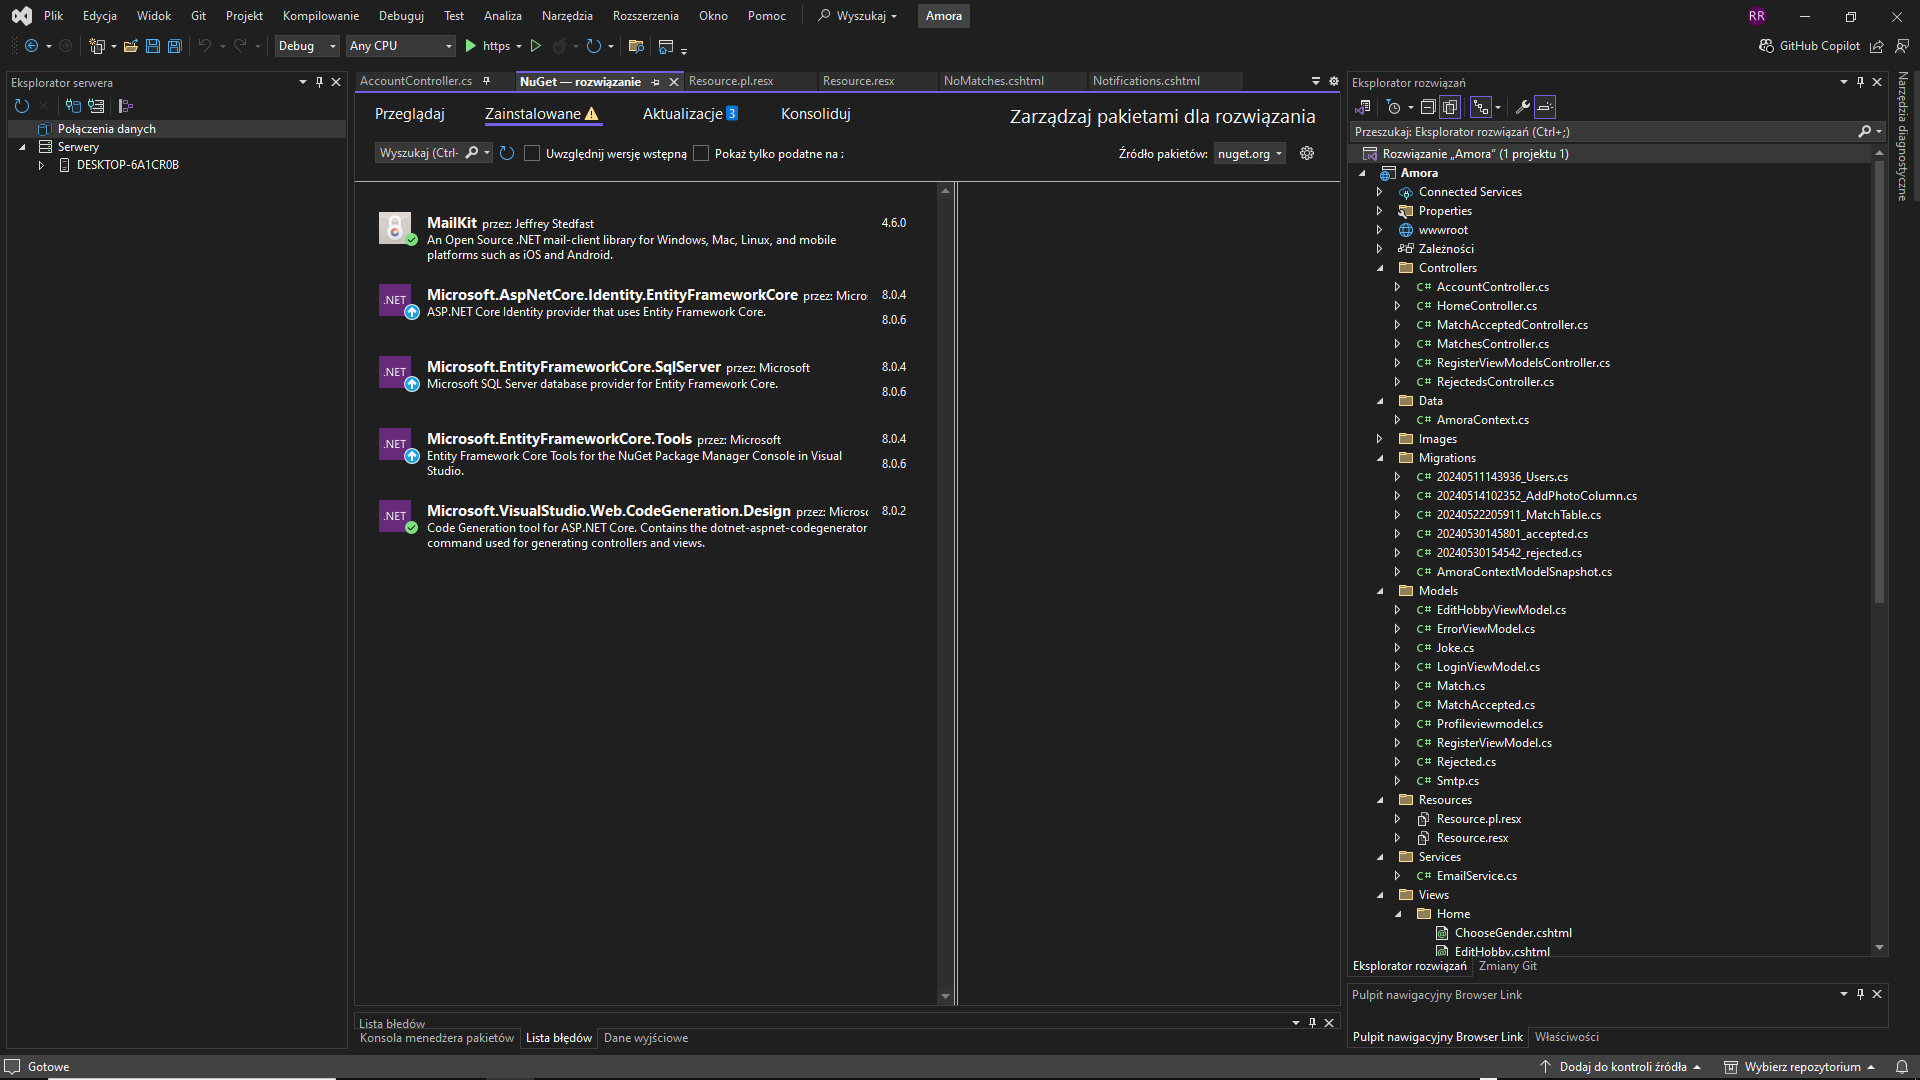
\includegraphics[width=1.0\linewidth]{images/10}
	\caption{}
	\label{fig:10}{Zależności projektu}
\end{figure}



\noindent
Użytkownicy platformy mogą: 
\begin{itemize}
	\item wybrac język platformy: angielski albo polski
	\item zarejestrować się 
	\item  utworzyć profil 
	\item  szukać dopasowań (wyborów potencjalnego partnera) - "match'y" z innymi użytkownikami platformy
	\item  przeglądać poprzednie dopasowania - "matche'e" w zakladce "Previous Matches"
	\item  odnaleźć numer telefonu swojej pary i poprzez niego nawiązać kontakt. Do pomocy w rozmowie mogą wykorzystać kawały, które znajdują się w tej samej zakładce.
	\item  zapoznać się z odpowiedziami na najczęściej spotykane problemy, zapytania -  w  sekcji FAQ(Frequently Asked Questions). Sekcja ta jest dostępna również dla niezarejestrowanych użytkowników.
\end{itemize}

\chapter{Opis technologiczny}

\newpage
\begin{figure}
	\centering
	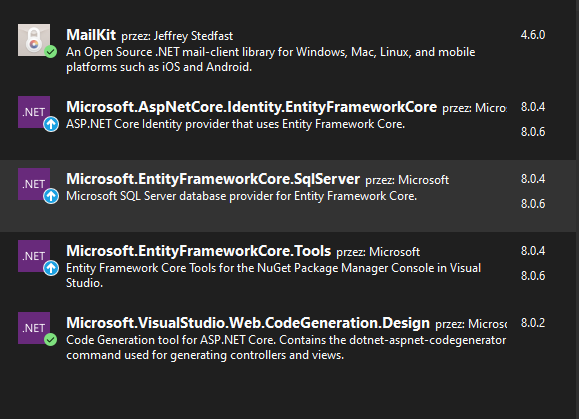
\includegraphics[width=1.1
	\linewidth]{images/screenshot001}
	\caption{}
	\label{fig:screenshot001}{Wymagane zależności w VSCommunity 2002}
\end{figure}

\noindent
Projekt zrealizowany w oparciu o:
 \begin{itemize}
 	\item relacyjną bazę danych  msSQL
 	\item  framework Microsoft.ASP.NetCore 8.0.0.0
 	zawierający pakiety:\\ MicrosoftASPNetCore.Identify.EntityFramework.Core wer. 8.0.4\\
 	Microsoft.Entity.FrameworkCore.Tools 8.0.4
 	\item framework do bazy - Microsoft.Entity.FrameworkCore.SQLServer 8.0.4
 	\item  framework CSS -bootstrap  wer. 5.1.0
 	\item biblioteka kliencka do poczty - MailKit 4.6.0
 \end{itemize} 	
 	
Wymagany system operacyjny w procesie projektowym, to  Windows 10 lub 11 z  zainstalowanym Microsoft ASP.NetCORE w wersji  8.0\\
Środowisko programistyczne oparliśmy na Visual Studio Community 2022 z skonfigurowanym menadżerem zależności NuGet. VSC pozwala obsłuje  język  \Csharp, pozwala na integrację z frameworkami i bazą danych, oferuje wszechstronne wsparcie dla języka C\# poprzez rozszerzenie C\# Dev Kit. Pozwala  na efektywną pracę z projektami .NET, w tym ASP.NET Core, Blazor czy aplikacjami konsolowymi. 
Aby zintegrować VS Code z frameworkiem, należy zainstalować odpowiednie rozszerzenia i skonfigurować środowisko pod kątem wymagań projektu.\\ 


	
\end{figure}

\section{Microsoft ASP.Net CORE wer. 8.0 - zestawienie modułów wykorzystanych w projekcie}
		 \noindent
		 System.Runtime 8.0.0.0\\
	     \noindent
		 Microsoft.Extensions.Options 8.0.0.0\\
		 Microsoft.Extensions.Options.ConfigurationExtensions 8.0.0.0\\
		 Microsoft.AspNetCore.HttpOverrides 8.0.0.0\\
		 Microsoft.Extensions.Configuration.Abstractions 8.0.0.0\\ 
		 Microsoft.AspNetCore.Routing 8.0.0.0\\\\
		 \noindent
		 Microsoft.Extensions.DependencyInjection 8.0.0.0\textbf{ wstrzykiwanie zależności}\\
		 Microsoft.Extensions.DependencyInjection.Abstractions 8.0.0.0\\
		 \noindent\\
		 Microsoft.AspNetCore.Http 8.0.0.0\\
		 Microsoft.AspNetCore.Http.Abstractions 8.0.0.0\\
		 Microsoft.AspNetCore.Serve.KestrelCore 8.0.0.0\textbf{ domyślny serwer HTTP}\\
		 \noindent\\
		 Microsoft.AspNetCore.HostFiltering 8.0.0.0\\
		 Microsoft.Extensions.Configuration 8.0.0.0\\
		 Microsoft.Extensions.Hosting 8.0.0.0\\
		 Microsoft.System.ComponentModel 8.0.0.0\\
		 Microsoft.Extensions.Features 8.0.0.0\\
		 \noindent\\
		 Microsoft.Extensions.Configuration.CommandLine 8.0.0.0\\
		 \noindent\\
		 Microsoft.AspNetCore.Hosting 8.0.0.0\\
		 Microsoft.Extensions.Hosting.Abstractions 8.0.0.0\\
		 Microsoft.AspNetCore.Hosting.Abstractions 8.0.0.0\\
		 Microsoft.AspNetCore.Hosting.Server.Abstractions 8.0.0.0\\
		 \noindent\\
		 Microsoft.Extensions.Configuration.EnvironmentVariables 8.0.0.0\\
		 Microsoft.Extensions.Configuration.Json 8.0.0.0\\
		 Microsoft.Extensions.Configuration.UserSecrets 8.0.0.0\\
		 \noindent\\
		 Microsoft.AspNetCore.Authentication.Abstractions 8.0.0.0\\
		 Microsoft.AspNetCore.Authentication 8.0.0.0\\
		 Microsoft.AspNetCore.Authorization 8.0.0.0\\
		 Microsoft.AspNetCore.Authorization.Policy 8.0.0.0\\
		 \noindent\\
		 Microsoft.Extensions.Logging 8.0.0.0\\
		 Microsoft.Extensions.Logging Abstractions 8.0.0.0\\ 
		 Microsoft.Extensions.Logging.Configuration 8.0.0.0\\
		 Microsoft.Extensions.Logging.Console 8.0.0.0\\
		 Microsoft.Extensions.Logging.Debug 8.0.0.0\\
		 Microsoft.Extensions.Logging.EventSource 8.0.0.0\\
		 \noindent\\
		 Microsoft.AspNetCore.Diagnostics 8.0.0.0\\
		 Microsoft.Extensions.Diagnostics.Abstractions 8.0.0.0
		 \noindent\\
		 System.Linq, Version=8.0.0.0\\
		 \pagestyle{plain}
\section{Zarządzanie zależnościami}
	Do zarządzania zależnościami - zarządca pakietów Nuget dla .NET - wykorzystywaliśmy go do wygodnego instalowania pakietów .NET poprzez Visual Studio Code Community. Pakiety były pobierane z repozytorium Microsoftu lub z repozytorium nugeta. Wymagało to jednak wstępnej konfiguracji w VSC(Visual Studio Code) i oczywiście uzyskaniu dostępu do tych repozytoriow - poprzez zarejestrowanie się na stronach www.nuget.org i potem konfiguracji VSC aby "widział" on te repozytoria podczas korzystania z manadżera pakietów NuGet \\ 
\section{Mapowanie}
	Do mapowania obiektowo-relacyjnego  (ORM) wykorzystujemy Entity Framework Core  z ASP.Net CORE. 
	Entity Framework umożliwia prace z danymi w bazie danych za pomocą obiektów i zapytań LINQ, co eliminuje potrzebę pisania bezpośrednich zapytań SQL.\\	 
\section{Technologie do budowy warstwy interfejsu użytkownika - frontend}
	 \noindent
	 Java Script\\
	 HTML\\
	 framework  CSS:  Bootstrap wer. 5.1.0\\
	 \pagestyle{plain}
\section{Cache}
	System cache jest implementowany przy użyciu wbudowanego w ASP.NETCore mechanizmu pamięci podręcznej\\
\newpage 

\chapter{Realizacja wymagań projektowych}
\newpage
\section{Wymagania projektowe i stopien realizacij}

\begin{table}[!htp]
	\centering
	\captionT{Lista zagadnień kwalifikacyjnych}
	%\begin{tabular}{|c|c|c|}
	\begin{tabular}{|c|c||p{7cm}|p{2ex}|}
		\hline
		Lp.&Zagadnienie&Opis&\\
		\hline
		1&framework MVC&wykorzystanie frameworka na backendzie&$\checkmark$\\
		\hline
		2&framework CSS&wykorzystanie frameworka na frontendzie&$\checkmark$\\
		\hline
		3& baza danych&dołączenie do projektu bazy danych&$\checkmark$\\
		\hline
		4&cache&dołączenie do projektu systemu cache&$\checkmark$\\
		\hline
		5&dependency manager& dołączenie do projektu systemu zarządzania zależnościami&$\checkmark$\\
		\hline
		6&HTML&szkielet aplikacji internetowej&$\checkmark$\\
		\hline
		7& CSS&ostylowanie aplikacji internetowej&$\checkmark$\\
		\hline
		8&JavaScript&uinteraktywnienie aplikacji internetowej&$\checkmark$\\
		\hline
		9&routing& wykorzystany routing i tzw. pretty URLs&$\checkmark$\\
		\hline
		10& ORM &wykorzystane mapowanie obiektowo-relacyjne&$\checkmark$\\
		\hline
		11&uwierzytelnianie&zaimplementowane mechanizmy nieuwierzytelnienia&$\checkmark$\\
		\hline
		12&lokalizacja&możliwość przełączania języka aplikacji&$\checkmark$\\
		\hline
		13&mailing&wysyłanie mejli z aplikacji&$\checkmark$\\
		\hline
		14& formularze& przesyłanie danych do aplikacji przez formularze&$\checkmark$\\
		\hline
		15&asynchroniczne interakcje& zaimplementowane asynchroniczne interakcje z serwerem&$\checkmark$\\
		\hline
		16&konsumpcja API& wykorzystanie zewnętrznego API&$\checkmark$\\
		\hline
		17&publikacja API&responsywny frontend&x\\
		\hline
		18&RWD& responsywny frontend&$\checkmark$\\
		\hline
		19&logger& logowanie akcji w systemie&$\checkmark$\\
		\hline
		20&deployment&  wdrożenie aplikacji internetowej&x \\
		\hline	
	\end{tabular}
	\label{tab_kwalifikacyjne}
\end{table}
\thispagestyle{plain} %przywraca numeracje
\newpage
\noindent Zrealizowane zagadnienia kwalifikacyjne wykonane według założeń z Tabela 4.1\\
\begin{enumerate}[label=\arabic*.,leftmargin=*]
	\item Framework MVC: Wykorzystujemy framework ASP.NET Core MVC do budowy backendu aplikacji: 
		\begin{itemize}
			\item (Model) Model danych - opis struktur danych i powiązań pomiędzy nimi
			\item (View) Interfejs, czyli to co widzi użytkownik
			\item (Controller) Logika działania - powiązania między zdarzeniami zachodzącymi w systemie
		\end{itemize}
	\item Framework CSS: Do stylizacji interfejsu użytkownika używamy frameworka Bootstrap. Bootstrap to popularny framework front-endowy, który zapewnia zestaw narzędzi, komponentów i stylów CSS.
	\item Baza danych: Projekt wykorzystuje Microsoft SQL jako bazę danych.
	\item Cache: Wdrożono mechanizm pamięci podręcznej do optymalizowania aplikacji.
	System Cache jest wykorzystywany w naszym projekcie do zapisywania oraz wyświetlania danych z profilu użytkownika tak aby za każdym najciemniej profil projekt nie musiał na nowo pobierać danych z bazy danych.
	\item Dependency manager: Do zarządzania zależnościami aplikacji używamy menedżera pakietów NuGet.
	NuGet jest menedżerem pakietów dla platformy .NET, który umożliwia łatwe dodawanie, usuwanie i aktualizowanie zależności bibliotek i narzędzi do projektów, co ułatwia zarządzanie zależnościami i zapewnia ponowne wykorzystanie kodu.
	\item HTML: Szkielet aplikacji internetowej został zbudowany zgodnie z standardami HTML.HTML służy do strukturyzowania treści na stronach internetowych poprzez definiowanie rożnych elementów, takich jak nagłówki, paragrafy, listy, obrazy, linki etc.
	\item CSS: Wykorzystujemy arkusze stylów CSS do ostylowania aplikacji.
	W naszej aplikacji korzystaliśmy z CSS do m.in. dodawania zdjęcia w tle strony, oraz do dokładniejszej konfiguracji wyglądu strony.
	\item JavaScript: W aplikacji użyto JavaScript do uinteraktywnienia interfejsu użytkownika.W naszym projekcie JavaScript używany jest do dodania wyskakującego okna z potwierdzeniem chęci wylogowania się oraz przy dodawaniu zdjęcia podczas rejestracji.
	\item Routing: Wykorzystujemy routing i tzw. pretty URLs dla estetycznych adresów URL.
	\item ORM: Do mapowania obiektowo-relacyjnego używamy Entity Framework Core.
	Entity Framework umożliwia prace z danymi w bazie danych za pomocą obiektów i zapytań LINQ, co eliminuje potrzebę pisania bezpośrednich zapytań SQL.
	\item Uwierzytelnianie: Uwierzytelnianie akcji w systemie polega na identyfikacji zalogowanego użytkownika przez system, co pozwala mu dostosować działania i udostępnić odpowiednie funkcjonalności zgodnie z jego uprawnieniami.
	\item Lokalizacja: W banerze strony jest opcja wyboru języka, pomiędzy polskim a angielskim. Do tłumaczenia strony korzystaliśmy z plików o rozszerzeniu .resx
	\item Mailing: Mailing to proces wysyłania wiadomości e-mail z aplikacji internetowej do określonych użytkowników lub grupy odbiorców. Używamy SMTP do wysyłania powiadomienia o  utworzonym koncie. Mamy również możliwość wysłania mejla ze zgłoszeniem.
	\item Formularze: Formularze to interaktywne elementy interfejsu użytkownika, które umożliwiają użytkownikom przesyłanie danych do aplikacji poprzez wprowadzanie informacji w pola tekstowe, wybieranie opcji, czy przesyłanie plików.
	Korzystamy z formularze poprzez rejestracje, logowanie, wybór płci, matchu, wysyłanie zgłoszenia oraz edycji hobby.
	\item Asynchroniczne interakcje: 
	Są procesami, w których zadania i odpowiedzi miedzy klientem a serwerem odbywają się niezależnie, umożliwiając wykonywanie innych operacji w trakcie oczekiwania na odpowiedz. Używamy ich podczas wrzucania zdjęcia podczas rejestracji oraz podczas wysyłania e-maila.
	\item Konsumpcja API: Konsumpcja API polega na pobieraniu danych lub wykonywaniu operacji z zewnętrznego interfejsu programistycznego. Korzystamy z Jokes API które generuje losowe żarty.
\end{enumerate}
	18. RWD: Responsywny front-end to taki, który automatycznie dostosowuje się do rożnych rozmiarów i typów urządzeń, zapewniając optymalne doświadczenie użytkownika na każdym ekranie.Mamy go za prawie za darmo stosując Bootstrapa.\\
\chapter{Instrukcja lokalnego i zdalnego uruchomienia}
\section{Instrukcja lokalnego uruchomienia systemu}
\begin{enumerate}
	\item Zainstaluj ASP.NET Core wer. 8.0  
	\item Zainstaluj Visual Studio Community 2022. Zarejestruj się na stronie www.nuget.org abyś mógł pobierać z repozytorium zależnosci i pakiety .NET poprzez menadżera pakietow Nuget w VSC. Skonfiguruj VSC do pobierania pakietow  z repozytoriów NuGet-a i Microsoft-u.
	\item Pobranie kodu źródłowego: Sklonuj repozytorium z Git Huba na swój lokalny komputer. Możesz to zrobić za pomocą polecenia git clone [adres repozytorium].Repozytorium projektu
	\item Otwarcie projektu: Otwórz pobrany projekt uruchamiając plik Amora.sln w wybranym edytorze kodu,na przykład Visual Studio Code lub innym.
	\item Instalacja zależności: Upewnij się, ze zainstalowane są wszystkie zależności projektu. Możesz to zrobić za pomocą menadżera pakietów NuGet. W konsoli NuGet należy wpisać komendę update-database.
	\item Uruchomienie aplikacji: Uruchom projekt poprzez ctrl+F5(Visual Studio) lub poprzez odpowiadająca opcje w innym edytorze.
	\item Otwarcie w przeglądarce: Po zakończeniu procesu uruchamiania projekt będzie dostępny pod adresem http://localhost:port.
	\item Testowanie funkcjonalności: Przetestuj rożne funkcje aplikacji, takie jak logowanie, rejestracja, przeglądanie profili, itp., aby upewnić się, że aplikacja działa poprawnie.
\end{enumerate}

\chapter{Rozmieszczenie dokumentacji i plików projektu na git-hubie}

\noindent
Strona projektu "AMORA"~~na github-ie:\\

https://github.com/jakubtrznadel/PipsiProject\\

\noindent
Pliki żródłowe "AMORA": w katalogu AMORA\\  
\noindent
Piki dokumentacji: w katalogu AMORADOCU\\

\chapter{Wnioski projektowe}

Korzystanie z .NET było fascynującym doświadczeniem, choć nie obyło się bez wyzwań, szczególnie podczas pierwszych kroków z Frameworkiem MVC. Metoda prób i błędów była naszą codziennością, a każde napotkane trudności stawały się szansą na naukę. Odkrywanie Frameworka CSS - Bootstrap-a stanowiło niezwykle interesująca cześć projektu, oferując narzędzia, których wcześniej nie mieliśmy okazji używać, co znacząco ułatwiło rozwój naszego projektu. Podsumowując, choć okres pracy był wymagający, zdobyte doświadczenie pozostanie z nami na długo,
pozostawiając nam cenne lekcje na przyszłość.

Platforma ASP.NET Core MVC udostępnia funkcjonalności, które znacznie ułatwiają tworzenie internetowych interfejsów API i aplikacji internetowych.
Jesteśmy zgodni w tym, że model MVC w ASP.NET Core wraz z mechanizmem wstrzykiwania zależności znacznie ułatwia projektowanie aplikacji internetowych i że od tej mamy inne spojrzenie na problematykę tworzenia portali internetowych.
Nie zdążyliśmy jeszcze dokonać publikacji API. Mamy nadzieję, że i to doświadczenie nie ominie nas w dalszym etapie nauki.   

\begin{comment}
%--------------------------------------------
%wykaz literatury
\renewcommand{\bibname}{Literatura}
\bibliographystyle{plabbrv}
\bibliography{references}
%--------------------------------------------

% --------------------------------------------
% Spis rysunków (odkomentować jeśli potrzeba)
%\listoffigures
%\addcontentsline{toc}{chapter}{Spis rysunków}
% --------------------------------------------

% --------------------------------------------
% Spis rysunków (odkomentować jeśli potrzeba)
%\listoftables
%\addcontentsline{toc}{chapter}{Spis tabel}
% --------------------------------------------

% --------------------------------------------
% Spis kodów źrodlowych (odkomentować jeśli potrzeba)
%\renewcommand\lstlistlistingname{Spis kodów źródłowych}
%\lstlistoflistings
%\addcontentsline{toc}{chapter}{Spis kodów źródłowych}
% --------------------------------------------

% --------------------------------------------
% Oswiadczenie - podpis
% --------------------------------------------
\newpage\thispagestyle{empty}
\par\vspace{1cm}\par
\begin{flushright}
....................................... \ \ \ \ \ \ \\
{\scriptsize (podpis)\hspace{2.3cm}\ }
\end{flushright}
\end{comment}
\end{document}